\documentclass[twocolumn, 12pt]{article}    % two-column because cheat sheets fit like that
\usepackage{preamble}

\begin{document}
\RaggedRight
\footnotesize % small because, it's a cheat sheet after all, why not cram it
\section*{Vibrations}



\begin{equation*}
    u(t) = u_c(t) +u_p(t) = \text{ total response}
\end{equation*}
\begin{equation*}
    m\ddot{u} + c\dot{u} + ku = F(t) \hspace{10pt}
    \Longrightarrow \hspace{10pt}
    \ddot{u} + 2\zeta\omega_n\dot{u} + \omega_n^2u = \frac{F(t)}{m}
\end{equation*}
\begin{equation*}
    \zeta = \frac{c}{2m\omega_n} \hspace{30pt}
    \omega_n = \sqrt{\frac{k}{m}} \hspace{30pt}
    \omega_d = \omega_n\sqrt{1-\zeta^2}
\end{equation*}


\noindent
\subsubsection*{Standard Form Conversions}
\[u(t) = 
\begin{cases}
    & 1) \hspace{15pt} B\cos(\omega t) + D\sin(\omega t)  \\
    & 2) \hspace{15pt} A\cos(\omega t + \phi) \\
    & 3) \hspace{15pt} C_1e^{j\omega t} + C_1^* e^{-j\omega t}\\
    & 4) \hspace{15pt} \mathrm{Re}\{Ce^{j\omega t}\}
\end{cases}
\vspace{-20pt} 
\]
\begin{table}[h!]
    \renewcommand\arraystretch{1.5}
    \centering
    \footnotesize
    \begin{tabular}{l|ll}
    \hline
        \multirow{2}{*}{1) - 2)} & \(B= A\cos(\phi)\) & \(D = -A\sin(\phi)\)\\
         & \(A = \sqrt{B^2 +D^2} \) & \( \phi = \text{atan2}(-D,\,B)\)\\
         \hline
         \multirow{2}{*}{1) - 3)} & \(B=2\mathrm{Re}\{C_1\} \) & \( D = -2\mathrm{Im}\{C_1\}\)\\
         & \(C_1 =\frac{1}{2}B - \frac{1}{2}jD\) & \\
         \hline
         \multirow{2}{*}{1) - 4)} & \(B = \mathrm{Re}\{C\} \) & \(D = -\mathrm{Im}\{C\}\) \\
         & \(C = B-jD\) & \\
         \hline
         \multirow{2}{*}{2) - 3)} & \(A =\sqrt{2}\left| C_1\right| \) & \(\phi = \text{atan2}(\mathrm{Im}\{C_1\},\,\mathrm{Re}\{C_1\})\)\\
         & \(C_1=\frac{A}{\sqrt{2}}e^{j\phi}\) & \\
         \hline
         \multirow{2}{*}{2) - 4)} &\(A = |C| \) &\( \phi = \text{atan2}(\mathrm{Im}\{C\},\,\mathrm{Re}\{C\})\)\\
         & \(C =Ae^{j\phi}\) & \\
         \hline
         3) - 4) & \(C=2C_1 \) & \( C_1=C/2\)\\
         \hline
    \end{tabular}
\end{table}
\vspace{-30pt} 
\subsubsection*{Solutions}
Standard 2\(^\text{nd}\) order:
\begin{equation*}
    u_c(t) = C_1e^{\lambda_1 t} + C_2e^{\lambda_2 t} \hspace{25pt} u_p(t) = \text{matches order of forcing}
\end{equation*}
\begin{equation*}
    \lambda_{1,2} = -\zeta \omega_n \pm \omega_n\sqrt{\zeta^2-1} = -\zeta\omega_n \pm j\omega_d \in \mathds{C}
\end{equation*}
Free and Undamped:
\[ u(t) = \begin{cases}
        &Ce^{j\omega_n t}+C^*e^{-j\omega_n t}\\
        &u_0\cos(\omega_n t) +\frac{\dot{u}_0}{\omega_n}\sin(\omega_n t)
 \end{cases}
 \hspace{30pt} \lambda_{1,2} \in \mathds{C} \setminus \mathds{R}
\]
Underdamped:
\begin{equation*}
    u_p(t) = e^{-\zeta\omega_n t} \left(a\cos(\omega_d t) +b\sin(\omega_d t) \right) = e^{-\zeta\omega_n t}\cos(\omega_d t +\phi)
\end{equation*}
\begin{equation*}
    T_d =\frac{2\pi}{\omega_d} \hspace{30pt} \left(\frac{\omega_d}{\omega_n}\right)^2 + \zeta^2 = 1 \hspace{30pt} \lambda_{1,2} \in \mathds{C}
\end{equation*}
Overdamped:
\begin{equation*}
    u_p(t) = C_1e^{\lambda_1 t} + C_2e^{\lambda_2 t} \hspace{30pt} \lambda_{1,2} \in \mathds{R} 
\end{equation*}
\[
\begin{cases}
    u(t=0) = u_0 = C_1 + C_2\\
    \Dot{u}(t=0) = v_0 =\lambda_1 C_1 + \lambda_2 C_2
\end{cases}
\]
Critically Damped:
\begin{equation*}
    u_p(t) = C_1 e^{\lambda t } + C_2 te^{\lambda t} \hspace{17.5pt} \lambda_{1,2}\in \mathds{R} \hspace{17.5pt} t \because \text{ ic's bad otherwise}
\end{equation*}
Harmonic Excitation:
\begin{equation*}
    u_p(t) = A(\omega) \cos(\omega t + \phi(\omega)) \hspace{30pt} A(\omega) \text{ implies } A(\omega) \in \mathds{R}_+
\end{equation*}
\[
\text{FRF} \triangleq \frac{A(\omega)}{F_0} \hspace{30pt}
\Omega \triangleq \frac{\omega}{\omega_n} \begin{cases}    
    &\in (0, \,1) \hspace{15pt} \phi(\Omega) = 0\\
    & =1 \hspace{32.5pt} \text{Resonance}\\
    &>1 \hspace{32.55pt} \phi(\Omega) = \pi
\end{cases}
\]
\begin{equation*}
    u_p(t,\Omega) = \frac{F_0}{m\omega_n^2} \frac{1}{1-\Omega^2}\cos(\omega t)
\end{equation*}
\begin{center}
Note: Resonance grows linearly with time.
\end{center}

\subsubsection*{Equation of Motion}
\begin{itemize}
    \item Newton's Law - FBD - \(\sum F = m\ddot{u}\)
    \item Euler's Law - FBD - \(\sum  M = J\ddot{\theta}\)
    \item Energy Conservation \(KE + PE =\) const \\ (dissipation not covered)
    \item Lagrangian \(L=KE-PE\), \,\(\frac{d}{dt}\left( \frac{\partial{L}}{\partial{\Dot{q}}}\right) - \frac{\partial{L}}{\partial{q}} =0\)  \(\forall q\) \\ (dissipation not covered)
\end{itemize}

\subsubsection*{Fourier Series}
\begin{equation*}
    f(t) = \sum_{n=0}^\infty  a_n\cos (n\omega t) + \sum_{n=1}^\infty b_n\sin(n \omega t) \hspace{25pt}T = 2\pi\omega
\end{equation*}
\begin{equation*}
    a_n = \frac{\omega}{\pi}\int_0^T f(t) \cos(n \omega t)dt \hspace{20pt} b_n = \frac{\omega}{\pi}\int_0^T f(t) \sin(n \omega t)dt
\end{equation*}
\(a_n\) and \(b_n\) are inner products with each of the sinusoidal bases

\subsubsection*{General Excitation}
\[
f(t) = \begin{cases}
    &1)\text{   Polynomial}\\
    &2)\text{   Harmonic}\\
    &3)\text{   Periodic \(\rightarrow\) Fourier Series}\\
    &4)\text{   Impulse}\\
    &5)\text{   Aperiodic \(\rightarrow\) Convolve}
\end{cases}
\]
Impulse: \hspace{120pt} equivalent forms
\begin{equation*}
    m\ddot{h} +c\dot{h}+kh = \delta(t), \hspace{30pt} h(0)=0, \hspace{10pt}  \dot{h}(0)=0
\end{equation*}
\begin{equation*}
    m\ddot{h} +c\dot{h}+kh = 0, \hspace{38pt} h(0)=0, \hspace{10pt} \dot{h}(0)=1/m
\end{equation*}
\begin{equation*}
    \text{\textbf{if   }} \zeta \in (0,\,1) \hspace{30pt} h(t) = \frac{1}{m\omega_d}e^{-\zeta \omega_n t}\sin(\omega_n t)
\end{equation*}
Convolution:
\begin{equation*}
    u_p(t) = g(t) \ast h(t) = \int_0^tg(\tau) h(t-\tau)d\tau \hspace{30pt} g(t) = \text{any}
\end{equation*}


\subsection*{MDOF}
\noindent \underline{Eigenfrequencies}: \(\{\omega_i\}\) \hspace{30pt} \underline{Eigenvalues}: \(\{\omega_i^2\}\)\\
\underline{Mode shapes}: Mass-normalized eigenvectors form an orthonormal basis (in modal space) of all possible vibrations
\begin{equation*}
    \vec{u}_i = \alpha_i \begin{bmatrix}
        u_{i1} & \dots & u_{in}
    \end{bmatrix}^T \hspace{20pt} \vec{u}_i^T M \vec{u}_i = 1 \hspace{20pt} \vec{u}_i^T K \vec{u}_i = \omega_i^2
\end{equation*}


\subsubsection*{Undamped}
\begin{enumerate}
    \item Solve transient/complementary \(\hspace{5pt} \vec{x} = \vec{u} e^{j\omega t}\) \hspace{5pt}\(\vec{u} \in \mathds{C}^n\)
    \begin{equation*}
        M\ddot{\Vec{x}} + K\Vec{x} = \Vec{0} \hspace{30pt} \text{char eq: } \det(K-\omega^2M) = 0 
    \end{equation*}
    \begin{equation*}
        \text{eigenvalues: } \{\omega_i^2\}  \hspace{30pt}  \text{eigenvectors: } \{\Vec{u}_i\} 
    \end{equation*}
    \begin{equation*}
        \text{Modal matrix: } U = \begin{bmatrix}
            \vec{u}_1 & \dots & \vec{u}_n
        \end{bmatrix} 
    \end{equation*}
    \begin{equation*}
        \begin{bmatrix}
            \vec{u}_1 & \dots & \vec{u_n}
        \end{bmatrix},\, \text{diag} (\lambda_1\, \dots \,\lambda_n) = \text{\mcode{eig}}(K,\, M)
    \end{equation*}

    \item Diagonalize into decoupled ODEs of modal coordinates
    \begin{equation*}
        \vec{x} = U\vec{q} \hspace{60pt} S = \text{diag} (\omega_1^2\, \dots\, \omega_n^2) 
    \end{equation*}
    \begin{equation*}
        \hspace{-10pt} U^TMU \ddot{\vec{x}} + U^TKU\vec{x} = U^T\vec{f}\sin(\omega t)
        \Longleftrightarrow I\ddot{\vec{x}} + S \vec{x} = \vec{g} \sin (\omega t)
    \end{equation*}
    Excitation of \(\vec{f}\) to mode \(i\) is \(|\vec{u}_j^T\vec{f}|\)

    \item Independently solve each SDOF modal ODE
    \begin{equation*}
        \ddot{q}_i  + \omega_j^2 q_i = g_i \sin (\omega t) \hspace{30pt} q_i(t) = q_{ic}(t) + q_{ip}(t)
    \end{equation*}

    \item Inverse transform to physical coordinates, and plug ics into \textbf{total solution} to solve for remaining undetermined complementary solution coefficients \(\vec{x} = U\vec{q}\)
\end{enumerate}

\subsubsection*{Proportional Damping}
Let/assert:  \(C = \alpha M + \beta K\) so that modal analysis can be used to find natural frequencies and mode shapes
\begin{enumerate}
    \item Ignore \(C\), find eigenvalues and eigenvectors
    \begin{equation*}
        \text{eigenvalues: } \{\omega_i^2\}  \hspace{30pt}  \text{eigenvectors: } \{\Vec{u}_i\} 
    \end{equation*}

    \item Diagonalize into decoupled ODEs of modal coordinates using \(U^T\)
    \begin{equation*}
        M\ddot{\vec{q}} + C \dot{\vec{q}} + K \vec{q} = \vec{f} \sin (\omega t)
    \end{equation*}
    \begin{equation*}
        I \ddot{\vec{q}}  + (\alpha I + \beta S) \dot{\vec{q}} + S \vec{q} = U^T \vec{f} \sin (\omega t) 
    \end{equation*}

    \item Compare to standard form to find damping
    \begin{equation*}
        \text{compare: } \begin{cases}
            \ddot{q}_i + (\alpha + \beta \omega_i^2) \dot{q}_i + \omega_i^2\vec{q} = (\vec{u}_i^T\vec{f}) \sin (\omega t)\\
            \ddot{q}_i + (2\zeta_i \omega_i) \dot{q}_i + \omega_i^2\vec{q} = (\vec{u}_i^T\vec{f}) \sin (\omega t)
        \end{cases}
    \end{equation*}
    With damping ratios: \hspace{15pt}  \(\zeta_i = \frac{1}{2}\left(\frac{\alpha}{\omega_i} +\beta \omega_i \right)\)

    \item Independently solve each SDOF modal ODE
    \begin{align*}
        q_i(t) &= q_{ic}(t) + q_{ip}(t)\\
        q_{ic}(t) &= e^{-\zeta_i \omega_i t} (A_1 \cos (\omega_d t) + A_2 \sin (\omega_d t)) \\
        q_{ic}(t) &= B_1 \cos (\omega t) + B_2 \sin (\omega  t)
    \end{align*}
    \begin{itemize}
        \item NOTE: Three frequencies present \(\{\omega, \omega_i, \, \omega_{id}\} \) (which assumes sys. is underdamped, otherwise \(\lambda_i = -\zeta_i\omega_i \pm \omega_i \sqrt{\zeta_i^1-1}\))
        \item Can use any form of harmonic motion eq. 
        \item \(A_1,\,A_2\) come from fitting to ics
        \item \(B_1,\,B_2\) are determined from particular sol.
    \end{itemize}

    \item Inverse transform to physical coordinates, and plug ics into \textbf{total solution} to solve for remaining undetermined complementary solution coefficients \(\vec{x} = U\vec{q}\)
\end{enumerate}

\subsubsection*{General (Non-Proportional) Damping}
\begin{enumerate}
    \item Solve transient/complementary 
    \begin{equation*}
        \text{let: } \vec{x}_c(t) = \vec{u} e^{\lambda t} \hspace{19pt} \vec{u} \in \mathds{C}^n \hspace{19pt} \det (\lambda^2 M + \lambda C + K) = 0
    \end{equation*}

    \item Solve for eigenvalues and eigenvectors (with \mcode{MATLAB}) 
    \begin{equation*}
        \begin{bmatrix}
            \vec{u}_1 & \dots & \vec{u_n}
        \end{bmatrix},\, \text{diag} (\lambda_1\, \dots \,\lambda_n) = \text{\mcode{polyeig}}(K, \,C,\, M)
    \end{equation*}
    \item Assemble complementary
    \begin{equation*}
        \vec{x}_c(t) = \sum_{i=1}^n \left( A_i \vec{u}_ie^{\lambda_i t}\right) + \underbrace{\text{complex conjugate}}_{\text{of sum at left}}
    \end{equation*}
    \(A_i\) are determined by fitting ics to \textbf{total response}

    \item  Solve for the particular solution
    Solve for \(\vec{x}_p(t)\) using the complex form, and take either the Real or Imaginary part of the solution to match to forcing function
    \begin{equation*}
        \text{let: } \vec{y}(t) = \vec{Y} e^{j\omega t} \hspace{30pt} \vec{Y} \in \mathds{C}^n \hspace{30pt} \omega = \text{driving freq.}
    \end{equation*}
    \begin{equation*}
        \vec{x}_p(t) = \begin{cases}
            \text{Im}\{\vec{y}(t)\} \hspace{15pt} \vec{f} \sim \sin\\
            \text{Re}\{\vec{y}(t)\} \hspace{15pt} \vec{f} \sim \cos\\
        \end{cases}
    \end{equation*}
    \begin{equation*}
        \hspace{-10pt}\vec{Y} = G(\omega) \vec{f}(t) \hspace{10pt}    G(\omega) = [-\omega^2M + j\omega C + K]^{-1} =\text{ FRF gain}
    \end{equation*}
    \begin{equation*}
        \hspace{-15pt} \vec{Y}(\omega) = \begin{bmatrix}
            |Y_1| e^{j \phi_1} \\ \vdots \\ |Y_n| e^{j \phi_n}
        \end{bmatrix} \hspace{10pt}
        \vec{x}_p(t) = \underbrace{\text{Im}\{ \vec{y}(t)\}}_{\text{Re\{\} for cos}} = \begin{bmatrix}
            |Y_1| \sin (\omega t + \phi_1) \\ \vdots \\ |Y_n| \sin (\omega t + \phi_n)
        \end{bmatrix}
    \end{equation*}
    \(|Y_i|,\, \phi_i\) are determined while fitting to the particular

    \item Plug ics into \textbf{total solution} to solve for remaining undetermined complementary solution coefficients \(A_i\)
\end{enumerate}



\subsubsection*{Vibration Absorber}
\begin{figure}[h!]
    \centering
    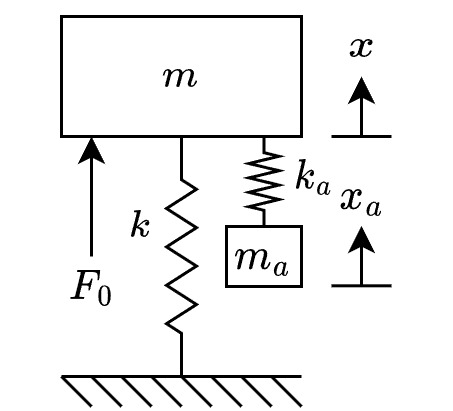
\includegraphics[width=.2\textwidth]{VibrationAbsorber.jpg}
\end{figure}
\begin{equation*}
    \begin{bmatrix}
        m  & 0 \\ 0 & m_a
    \end{bmatrix} \ddot{\vec{x}} + \begin{bmatrix}
        k+k_a & -k_a \\ -k_a  & k_a
    \end{bmatrix} \vec{x} = \vec{f} \sin(\omega t)
\end{equation*}
\begin{equation*}
    \vec{y}_p(t) = \vec{Y} e^{j \omega t} \Longrightarrow \vec{x}_p(t) = (-\omega^2M + K )^{-1}\vec{f} \sin(\omega t)
\end{equation*}
\begin{equation*}
    \vec{x}_p(t) = \frac{F_0 \sin (\omega t)}{\det (K-\omega^2M)} \begin{bmatrix}
        k_a - \omega^2 m_a \\ k_a
    \end{bmatrix}
\end{equation*}
\begin{equation*}
    (k_a-\omega^2 m_a) \to 0, \, x_{pm} \to 0 \text{ as desired!}
\end{equation*}




%\vspace{3 in}
\begin{center}
    \footnotesize Levi Barker \hspace{150pt} U0959362
\end{center}




\end{document}